\documentclass{article}
\usepackage{tikz}

\begin{document}

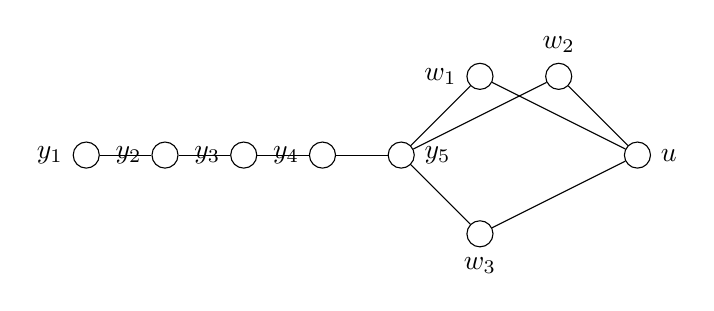
\begin{tikzpicture}[node distance=1cm]
    % Define the nodes
    \node[circle,draw] (y1) at (0,0) [label=left:$y_1$] {};
    \node[circle,draw] (y2) at (1,0) [label=left:$y_2$] {};
    \node[circle,draw] (y3) at (2,0) [label=left:$y_3$] {};
    \node[circle,draw] (y4) at (3,0) [label=left:$y_4$] {};
    \node[circle,draw] (y5) at (4,0) [label=right:$y_5$] {};
    \node[circle,draw] (w1) at (5,1) [label=left:$w_1$] {};
    \node[circle,draw] (w2) at (6,1) [label=above:$w_2$] {};
    \node[circle,draw] (w3) at (5,-1) [label=below:$w_3$] {};
    \node[circle,draw] (u) at (7,0) [label=right:$u$] {};

    % Draw the edges
    \draw (y1)--(y2);
    \draw (y2)--(y3);
    \draw (y3)--(y4);
    \draw (y4)--(y5);
    \draw (y5)--(w1);
    \draw (y5)--(w2);
    \draw (y5)--(w3);
    \draw (u)--(w1);
    \draw (u)--(w2);
    \draw (u)--(w3);
\end{tikzpicture}

\end{document}